\documentclass{article}
\usepackage{graphicx} % Required for inserting images
\usepackage[top=0.9in, bottom=1in, left=1.5in, right=1.5in]{geometry}
\usepackage[utf8]{inputenc}
\usepackage[icelandic]{babel}
\usepackage[T1]{fontenc}
\usepackage[sc]{mathpazo}
\usepackage[parfill]{parskip}
\renewcommand{\baselinestretch}{1.2}
% Tables and lists
\usepackage{booktabs,tabularx}
\usepackage{multirow}
\usepackage{enumerate}
\usepackage{adjustbox}
\usepackage{multicol}
\usepackage{xcolor}
\usepackage{algpseudocode}
\usepackage{algorithm}
\usepackage{tikz}
\usepackage{nicefrac}
\usepackage{changepage}
\usepackage{fancyvrb}
\usepackage{xlop}
\usetikzlibrary{arrows, positioning, calc, graphs}

% Math
\usepackage{amsmath, amsfonts, amssymb, amsthm}
% Graphics

\usepackage{graphicx}
\usepackage{tikz}
% Code environment
\usepackage{minted}
%\usepackage{bm}
%\usepackage{siunitx}
%\usepackage{animate}
%\usepackage{hyperref}
%\usepackage{movie15}
%\usepackage{multicol}
%\usepackage{changepage}
\title{Tölvutækni og forritun Heimadæmi 7}
\author{Ragnar Björn Ingvarsson, rbi3}
\tikzset{->, >=stealth', shorten >=1pt, node distance=2cm,thick, main node/.style={circle,draw,minimum size=3em}}


\begin{document}
\renewcommand\thepage{}
	
	\maketitle

	\newpage
	\setcounter{page}{1}
	\renewcommand\thepage{\arabic{page}}

	\section{}

	Við athugum að smalamálskóðinn virkar svo að hann fyrst ber saman \%esi 
	og \%edi og síðan, ef \%edi er minna eða jafnt og \%esi, þá hoppar 
	forritið í .L2 en annars heldur það áfram og klárar leyndo.

	Þegar það klárar leyndo setur það $\%rdx + \%rdi \cdot 2$ í \%eax og 
	skilar því gildi.

	Ef það hoppar í .L2 þá setur það $\%rsi \cdot 3$ í \%eax og plúsar \%edx 
	við það og skilar \%eax.

	Einnig er $a$ í \%rdi, $b$ í \%rsi og $c$ í \%rdx.

	Svo C kóðinn er 

	\begin{verbatim}
int leyndo(int a, int b, int c)
{
    if (a > b)
        return c + 2*a;
    else
        return c + b*3;
}
	\end{verbatim}

	\section{}

	\begin{itemize}
		\item[a)] Við köllum á pushq tvisvar fyrir \%rbp og \%rbx sem er þá 
			til að setja upprunalegu gildi þessara gista á hlaðann til að 
			vista þau svo að í lok fallsins getum við pop-að þeim af hlaðanum 
			svo gildin haldist eins fyrir og eftir fallið.
		\item[b)] Movq skipanirnar þjóna mismunandi tilgangi, fyrsta er til 
			að vista gildið $b$ í \%rbp sem leyfir okkur að vera viss um að 
			gildið breytist ekki eftir fyrsta kallið á xyz þar sem \%rbp 
			breytist ekki fyrir og eftir köll á föll.

			Næst færum við \%rax í \%rbx sem er gert þar sem \%rax er 
			skilagildi fallsins xyz í fyrsta kallinu, svo við viljum geyma 
			það skilagildi svo það yfirritist ekki af seinna kallinu. 

			Síðan færum við \%rbp í \%rdi sem er í raun að færa vistaða 
			gildið á $b$ inn í \%rdi sem er gistið sem notað er fyrir fyrsta 
			inntak falls. Svo þetta er gert til að setja $b$ sem inntak inn 
			í seinna kall á fallið xyz.
	\end{itemize}

	\section{}

	\begin{itemize}
		\item[a)] gcc virðist hætta að nota stökktöflu þegar við fækkum 
			tilfellunum um einn, svo tilfellin hætta að þurfa stökktöflu 
			þegar þau eru fækkuð niður í 4. Þetta er útkoman sama hvaða gildi 
			við berum $x$ við og er vegna þess væntanlega að gcc telur það 
			hagkvæmara að framkvæma þá bara nokkrar compare skipanir í stað 
			þess að búa til stökktöflu
			\begin{center}
				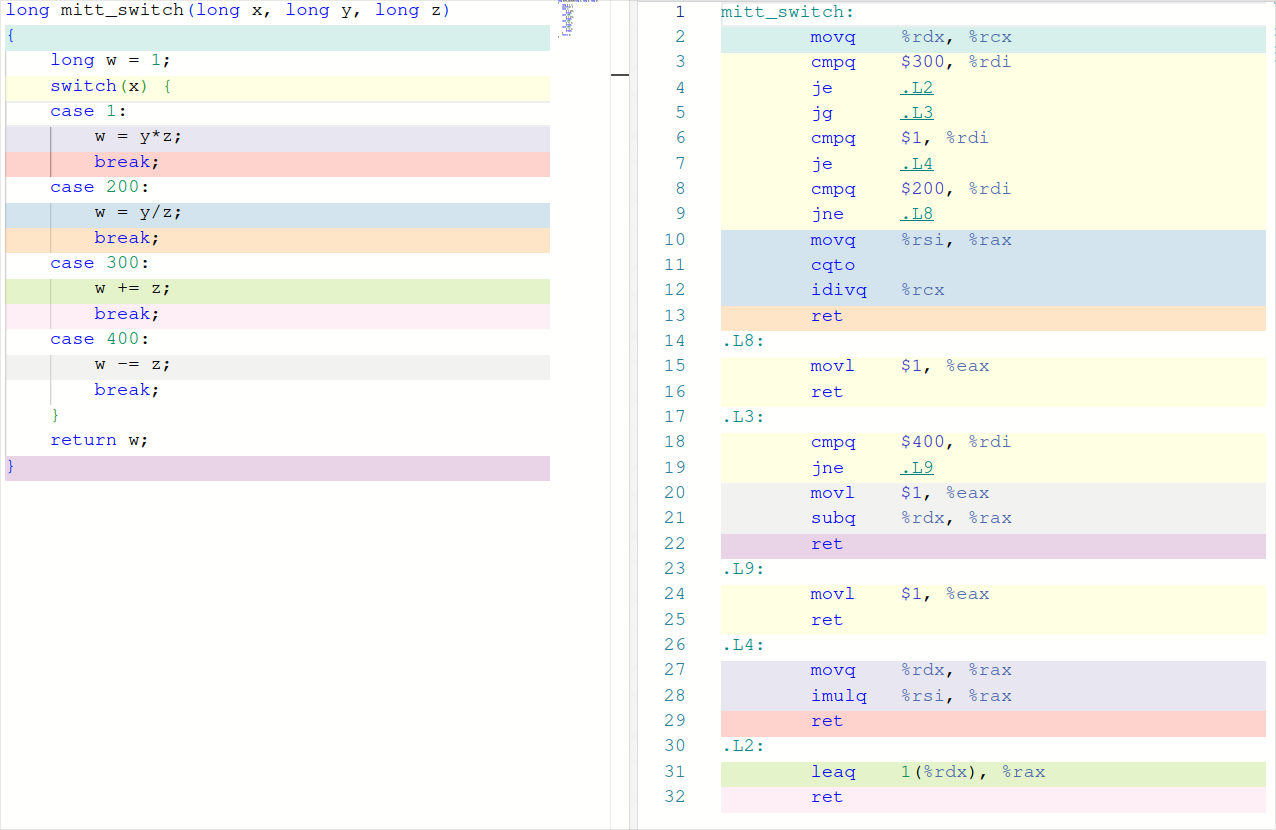
\includegraphics[scale=0.3]{less.png}
			\end{center}
		\item[b)] gcc hættir að nota stökktöflu fyrir öll gildi á tilfelli 5 
			sem eru hærri en 40, svo 40 er hæsta gildið sem gcc notar fyrir 
			stökktöfluna.
			\begin{center}
				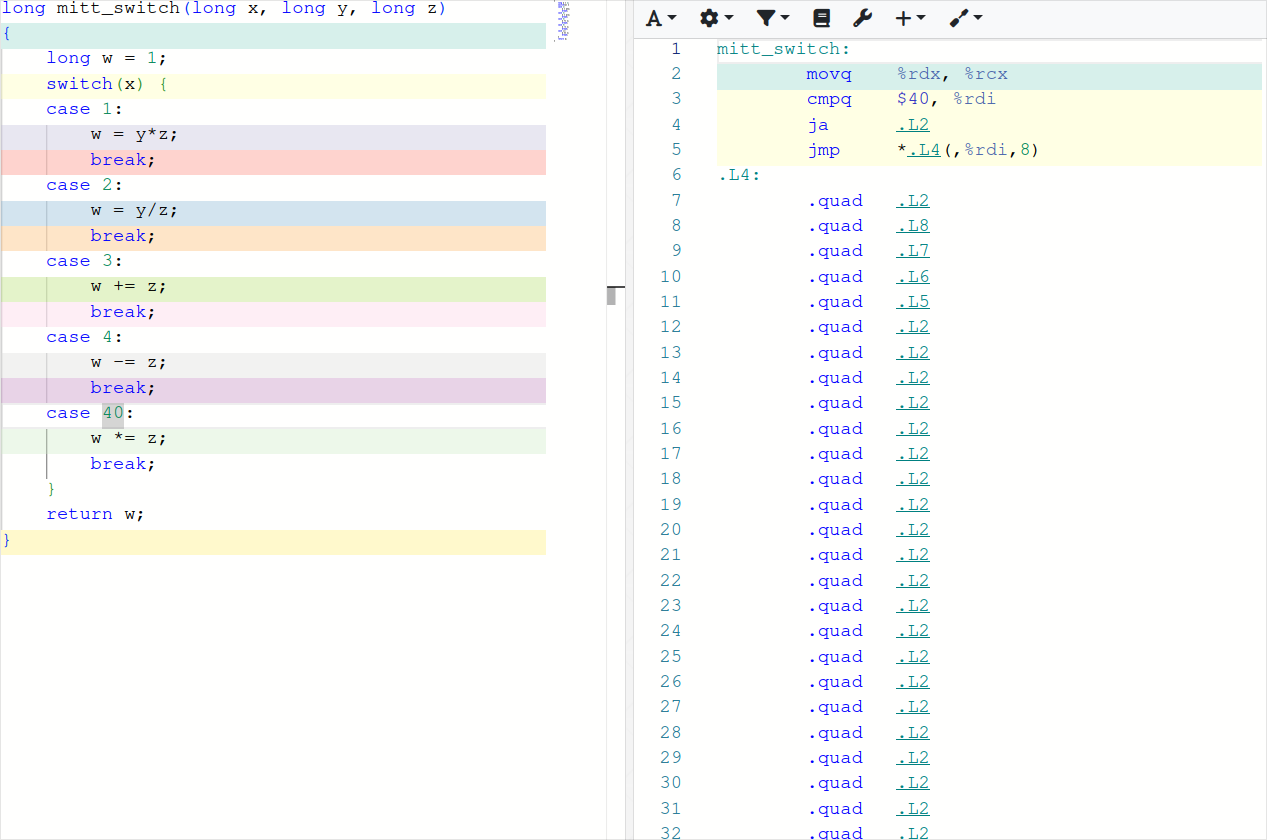
\includegraphics[scale=0.25]{highest.png}
				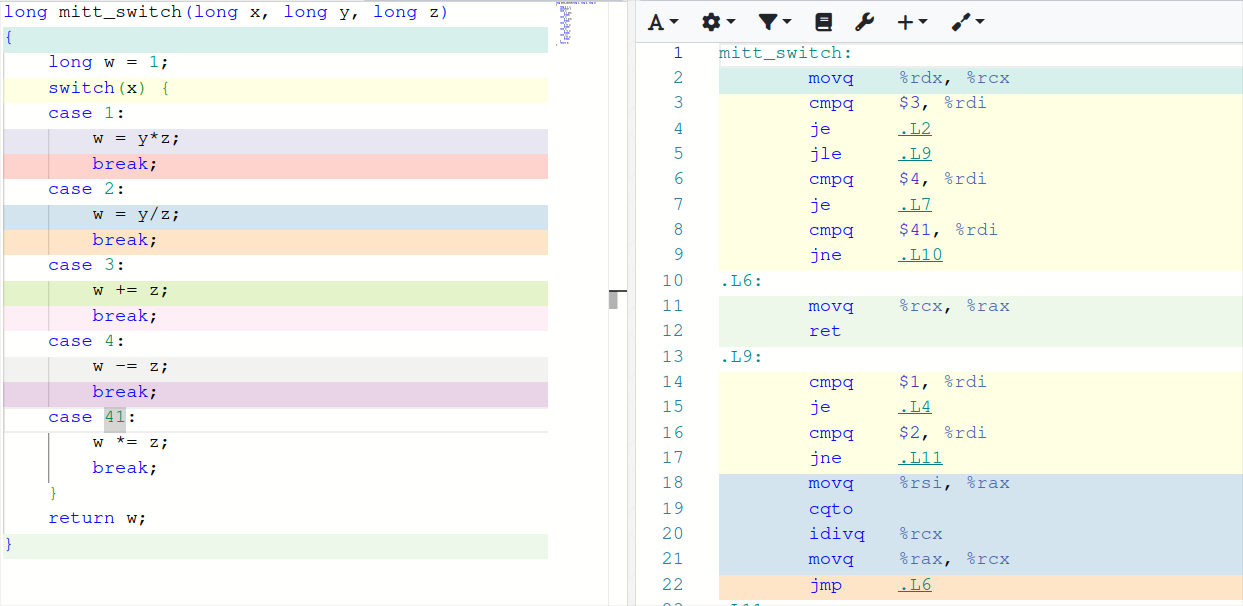
\includegraphics[scale=0.25]{over.png}
			\end{center}
		\item[c)] Ef við segjum að fyrsta tilfellið byrji þá á $-5$, ákveður 
			gcc að plúsa $5$ við $x$ og bera það saman við $10$. Svo gcc 
			tekur bilið sem verið er að prófa tilfelli á og ber $x$ saman við 
			það bil sem jákvæða tölu. Semsagt

			\begin{center}
				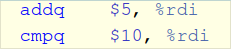
\includegraphics[scale=0.75]{add5.png}
			\end{center}
	\end{itemize}

	\section{}

	\begin{itemize}
		\item[a)] Við sjáum að fallið notar gistin \%rdi, \%rsi og \%rdx og 
			skilar svo \%rax. Svo fallið tekur þrjú inntök sem eru öll 
			\textbf{long}, þar sem alltaf er notuð r útgáfan en ekki e. 
			Einnig er fyrsta inntakið pointer þar sem náð er í gildið með (\%rdi)
		\item[b)] Veljum að inntökin séu a, b og c og að fallið skili x

			\begin{verbatim}
long fun(long *a, long b, long c)
{
    long x = *a;
    while (b < c) {
        x *= 6;
        b++;
    }
    return x;
}
			\end{verbatim}
	\end{itemize}

	\newpage
	\section{}

	\begin{itemize}
		\item[a)] Fallið í C lítur svona út
\begin{verbatim}
int rec(int n, int m)
{
    if (n >= m) { // comparator fyrir línur 1 og 2
        m+=m; // Lína 6
        n-=2; // Lína 7
        // Hérna sameina ég línur 8, 9 og 11, kallað er á fallið í línu 8, 
        // svo er einum bætt við skilagildi fallsins í línu 9 og skilað í línu 11.
        return rec(n,m) + 1;
    }
    return 0; // Ef hoppið gerist ekki, er jafnt línum 3 og 4
}
\end{verbatim}
		\item[b)] Við sjáum að stack frameið inniheldur alltaf return addressið efst og svo tökum við 8 frá $\%rsp$ til að búa til 8 bæta pláss sem er sér 
			fyrir fallið, en notum plássið ekkert í fallinu svo þetta lítur svona út:

			\begin{center}
				\begin{tabular}{ |c| }
					\hline
					8 bæta pláss \\
					\hline
				\end{tabular}
			\end{center}

			Þar sem $\%rbp$ bendir á MSB og $\%rsp$ bendir á LSB

	\end{itemize}

\end{document}
